\section{Design}

The Team Zero Chat Application system's design involves several parts, as shown in figure \ref{design}. 

The Team Zero Server is intended to run 24/7, along with the Postgresql database which is hosted on Heroku, a cloud platform.

This project involves two types of clients - Android and Web. However, this design will allow for extension to any type of client, provided the implementation meets the Server's API guidelines (see section \ref{api}). Both of the clients have web sockets with which they communicate with the server. The server's web socket accepts multiple web socket connections, and communicates with the database to retrieve and store information as required.

Although a client cannot send a message directly to another client without going through the server, this distributed chat system is considered end-to-end secure as the server does not interfere with or read the content of the message. Additionally, the content of the message will be encrypted.


\begin{figure}[H]
  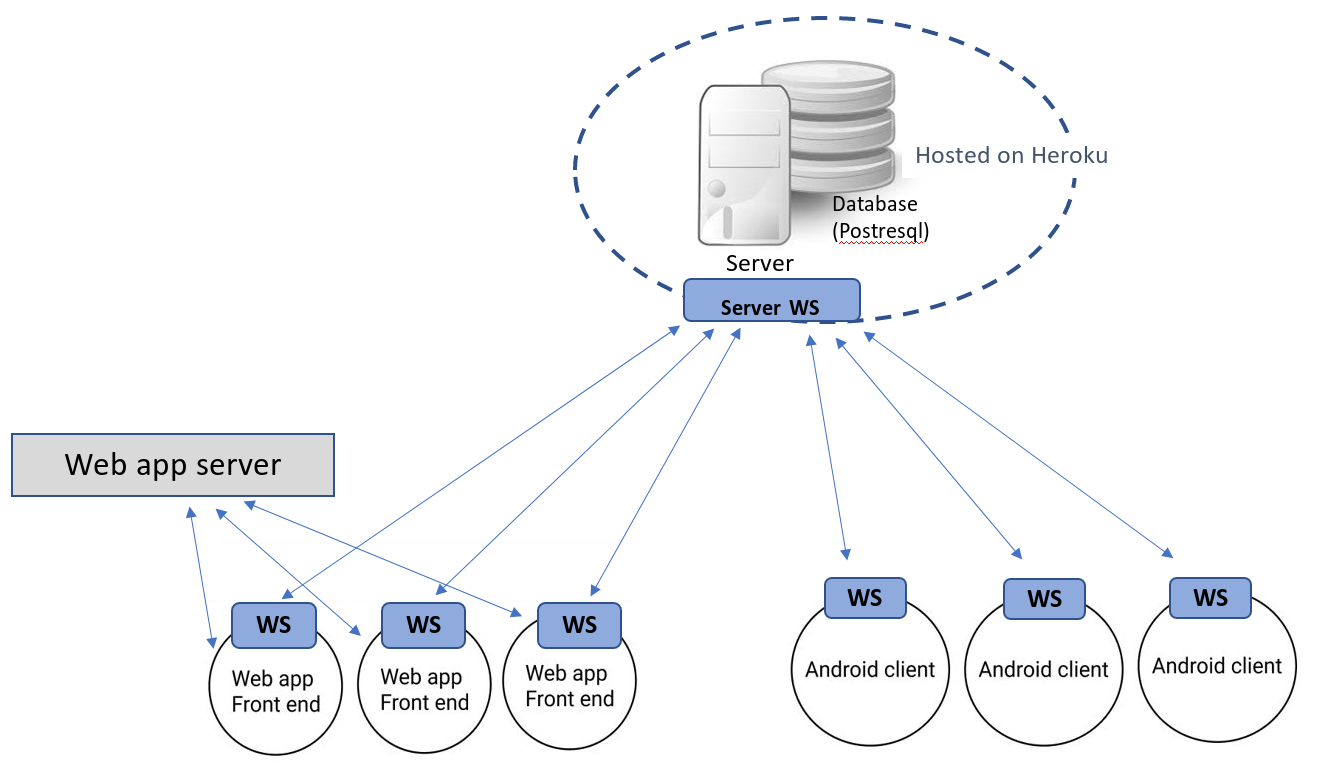
\includegraphics[scale=0.3]{images/design.png}
  \caption{The Team Zero Application}
  \label{design}
\end{figure}
